% This file was created by tikzplotlib v0.9.2.
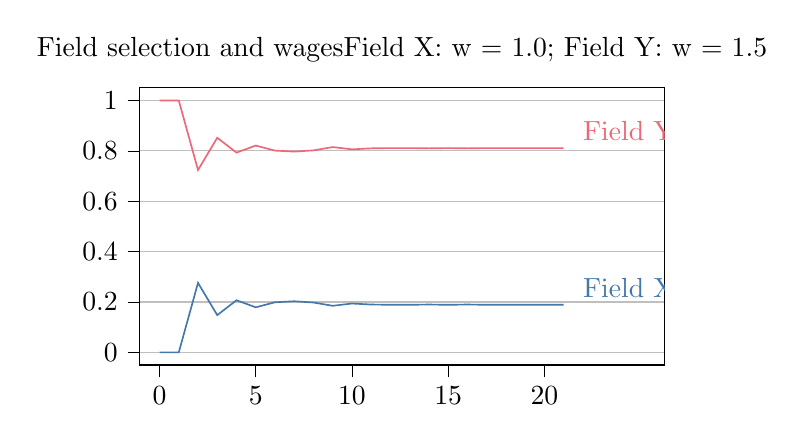
\begin{tikzpicture}

\definecolor{color0}{rgb}{0.266666666666667,0.466666666666667,0.666666666666667}
\definecolor{color1}{rgb}{0.933333333333333,0.4,0.466666666666667}

\begin{axis}[
height=5.101085673964669cm,
tick align=outside,
tick pos=left,
title={Field selection and wages \\ Field X: w = 1.0; Field Y: w = 1.5},
width=8.25373cm,
x grid style={white!69.0196078431373!black},
xmin=-1.05, xmax=26.25,
xtick style={color=black},
xtick={0,5,10,15,20},
xticklabels={\(\displaystyle 0\),\(\displaystyle 5\),\(\displaystyle 10\),\(\displaystyle 15\),\(\displaystyle 20\)},
ymajorgrids,
ymin=-0.05, ymax=1.05,
ytick style={color=black},
ytick={0,0.2,0.4,0.6,0.8,1},
yticklabels={\(\displaystyle 0\),\(\displaystyle 0.2\),\(\displaystyle 0.4\),\(\displaystyle 0.6\),\(\displaystyle 0.8\),\(\displaystyle 1\)}
]
\addplot [semithick, color0]
table {%
0 0
1 0
2 0.276
3 0.148
4 0.207
5 0.179
6 0.199
7 0.203
8 0.198
9 0.185
10 0.194
11 0.19
12 0.189
13 0.189
14 0.19
15 0.189
16 0.19
17 0.189
18 0.189
19 0.189
20 0.189
21 0.189
};
\addplot [semithick, color1]
table {%
0 1
1 1
2 0.724
3 0.852
4 0.793
5 0.821
6 0.801
7 0.797
8 0.802
9 0.815
10 0.806
11 0.81
12 0.811
13 0.811
14 0.81
15 0.811
16 0.81
17 0.811
18 0.811
19 0.811
20 0.811
21 0.811
};
\draw (axis cs:21.5,0.219) node[
  anchor=base west,
  text=color0,
  rotate=0.0
]{Field X};
\draw (axis cs:21.5,0.841) node[
  anchor=base west,
  text=color1,
  rotate=0.0
]{Field Y};
\end{axis}

\end{tikzpicture}
